\section{Query evaluation}

In this section, we explain how to evaluate queries with the given data set. For this query evaluation we can use a distributed event stream processing system with the process graph as shown in Figure \ref{twonode_graph} for both queries.

\begin{figure}[!t]
        \centering
        \includegraphics[width=2.0in]{twonode_graph.png}
        \caption{Two node process graph to evaluate queries}
        \label{twonode_graph}
\end{figure}

\textit{EventEmitter} reads the data file and generates events with a sequence number. This sequence number is used to order \textit{QueryEvaluator} results. For real implementation, each query has its own \textit{EventEmitter} that reads each line of the data file and generates an event with the relevant information. \textit{QueryEvaluator} evaluates the query against the received event and generates top ten value changed event.  In general we can evaluate queries sequentially and in parallel. In a sequential execution, all events goes to one \textit{QueryEvaluator} instance and in a parallel execution, the event stream is partitioned using the key field and evaluate simultaneously with different \textit{QueryEvaluator} instances.

\subsection{Sequential evaluation}

We can sequentially execute events either in a single Java Virtual Machine (JVM) or in different JVMs (either in one machine or different machines) using TCP sockets to communicate among process instances. Figure \ref{sequential} shows possible executions. 

\begin{figure}[!t]
        \centering
        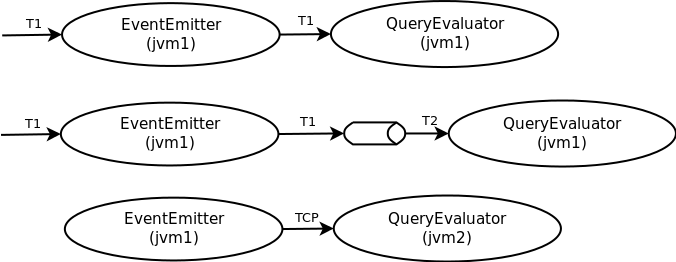
\includegraphics[width=3.0in]{sequential.png}
        \caption{Different types of sequential execution}
        \label{sequential}
\end{figure}

First both processors can be executed in same JVM with same thread. In that case, both processes execute sequentially. We can make two processes parallel by executing them with two threads and communicate using a queue in same JVM or communicate using a TCP connection for different JVMs. In all these cases \textit{QueryEvaluator} processes messages sequentially and becomes the bottleneck. Next we show how to parallel \textit{QueryEvaluator} process. 

\subsection{Parallel evaluation}
The general way to parallelize event processing, is to partition the events according to a key and run multiple instances to process data. Therefore in this section, we explain how to parallelize the query evaluation process taking frequent route query into consideration. Same concepts can be applied to profitable cell evaluation as well.

For frequent route query, route events can be partitioned using the hash code of the route object and process different route sets in different \textit{QueryEvaluators}. In such a setup, each \textit{QueryEvaluator} generates an event when the top ten routes get changed for its route set. Since this is not the desired result, we can add another process to aggregate these top result events and generate global route change events. Figure \ref{parallel} shows, possible parallel evaluation techniques with the new process. Multiple \textit{QueryEvaluator} instances can be executed in a single JVM using multiple threads or in a distributed setup with many JVMs using TCP to communicate. 

\begin{figure}[!t]
        \centering
        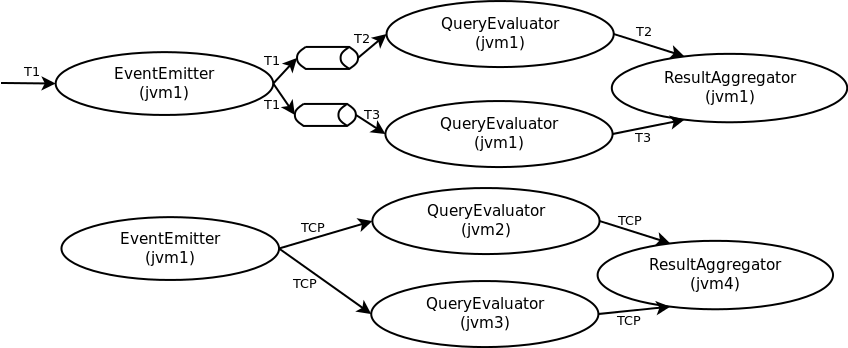
\includegraphics[width=3.0in]{parallel.png}
        \caption{Different types of parallel execution}
        \label{parallel}
\end{figure}

\textit{ResultAggregator} keeps a set of route counts received by \textit{QueryEvaluators}. Upon receiving a new event, it can update the existing route count values and check whether the global top ten route counts have changed. If there is a change, it can generate a top ten route changed event. This logic has the following issues and can be fixed as given bellow.

\begin{enumerate}
	\item \textbf{Expired values} : Route count of a particular route can be reduced due to expiration of some events. For an example, lets assume route count for route R1 is 10 and R1 is included in a top ten route event generated by a \textit{QueryEvaluator}. Then lets assume when the next event is generated, the route count for R1 has been reduced to 7 (due to expiration events) and hence R1 is not included in the next top ten route event. However since R1 value still is in the \textit{ResultAggregator} that may produce an event with this value. To avoid this problem, we send the removed route set details with the top ten route event generated by the \textit{QueryEvaluator}. In that case \textit{ResultAggregator} can first remove those routes.
	\item \textbf{Out of order events} : \textit{ResultAggregator} may receive events in a different order than those are produced at the \textit{EventEmitter}. This out of order events may change the final output of the \textit{ResultAggregator}. We order messages at the \textit{ResultAggregator} to avoid this problem. In order to order messages, we keep a message queue for each \textit{QueryEvaluator} and sent the message with least sequence number to \textit{ResultAggregator},  if a message is present in all queues. 
	\item \textbf{Intermediate top ten route events} : A route event increases the route count for that events' route. Further that can generate some expiration events which may reduce the route count for other routes. The top ten frequent routes can be changed due to these expiration events as well. Lets say in one \textit{QuerayEvaluator} case, a particular event causes two routes R1 and R2 to change and generates a top ten route change event. In the distributed setup these two routes can be in two \textit{QueryEvaluators} and that can cause two top ten route change events. These two events may result in two top ten route change events at \textit{ResultAggregator} as well instead of one. Further we observed only around 5\% of such events are generated, and system goes to the one \textit{QueryEveluator} result after all such event are being executed. Solution for such a problem may depend on the nature in which a real application, uses these results in decision making process. Therefore we could not provide any fix for this problem.
\end{enumerate}

Algorithm \ref{aggregate_algorithm} shows the algorithm for ResultAggregator with above fixes. First it removes the expired keys. Then it updates the existing values or adds new values and moves the position in the list accordingly. Finally it generates an event if there is a change to the top list.


\begin{algorithm}
\caption{Algorithm to aggregate top ten results from QueryEvaluators and generate global events}
\label{aggregate_algorithm}
\begin{algorithmic}

\STATE preTopTen $\leftarrow$ nodeList.getTopValues()
\FORALL {key in event.removedKeys}
	\STATE nodeList.remove(key)
\ENDFOR

\FORALL {nodeValue in event.newValuesList}
	\IF {nodeList.containsKey(nodeValue.key)}
		\STATE existingValue $\leftarrow$ nodeList.get(nodeValue.key)
		\IF { existing value is lesser than current }
			\STATE update the existing value
			\STATE nodeList.decrementPosition(nodeValue.key)
		\ELSE
			\STATE update the existing value
			\STATE nodeList.incrementPosition(nodeValue.key)
		\ENDIF
	\ELSE
		\STATE nodeList.add(nodeValue.key, nodeValue)
	\ENDIF
\ENDFOR

\STATE nowTopTen $\leftarrow$ nodeList.getTopValues()
\IF { preTopTen not equals nowTopTen }
	\STATE emit new event
\ENDIF
\end{algorithmic}
\end{algorithm}
